% ch03-ml.tex -- Supervised learning and honest evaluation
\chapter{Supervised learning and honest evaluation}\label{ch:eval}

Every supervised question collapses to two decisions: \emph{what are we
predicting}, and \emph{how will we know it worked}. This chapter installs the
whole frame --- dataset, model, loss, split, metric --- and powers it with the
two simplest classifiers in the canon: $k$-nearest neighbours\index{$k$-nearest
neighbours} (memorise, then vote) and na\"ive Bayes\index{na\"ive Bayes}
(multiply little probabilities, then compare). Neither needs a library call to
explain, so both get written from scratch below. The rest of the chapter is
about the harder discipline: evaluation. A number on held-out data, computed
under a protocol that never let the model peek, is the only currency this
book trades in. By the end you will have a harness --- split, fit, predict,
score --- that every later chapter reuses unchanged.

\section{The supervised problem}\label{sec:supervised}

\begin{definition}[Supervised dataset]\label{def:supervised}
A \emph{supervised dataset} is
$\mathcal D = \{(\mathbf{x}_i, y_i)\}_{i=1}^{n}$: $n$ pairs of a feature row
$\mathbf{x}_i \in \mathbb{R}^d$ and a label $y_i$. In the matrix view of
Chapter 1, $\mathcal D$ is an $X \in \mathbb{R}^{n\times d}$ together with a
$\mathbf{y} \in \mathbb{R}^{n}$ (regression) or $\mathbf{y} \in
\{0,1,\dots,C{-}1\}^{n}$ (classification).
\end{definition}

A \emph{model}\index{model} is a function
$f_{\boldsymbol\theta}: \mathbb{R}^d \to \hat{y}$ chosen from a family by
adjusting parameters $\boldsymbol\theta$ to fit $\mathcal D$. Training is the
fit; evaluation is checking the fit \emph{on rows the fit never saw}. That
last clause is the entire game, and the whole chapter turns on it.

\begin{figure}[ht]\centering
\begin{tikzpicture}[font=\small, node distance=0.55cm]
  \node[draw, rounded corners, minimum width=2.0cm, minimum height=0.9cm]
    (raw) {raw table $(n,d)$};
  \node[draw, rounded corners, right=of raw] (split) {split};
  \node[draw, rounded corners, right=of split] (fit) {fit on train};
  \node[draw, rounded corners, right=of fit] (pred) {predict on test};
  \node[draw, rounded corners, right=of pred] (score) {score once};
  \draw[->] (raw) -- (split);
  \draw[->] (split) -- (fit);
  \draw[->] (fit) -- (pred);
  \draw[->] (pred) -- (score);
  \node[below=0.25cm of fit, font=\scriptsize, align=center, text width=2.6cm]
    {parameters live here};
  \node[below=0.25cm of score, font=\scriptsize, align=center, text width=2.6cm]
    {the only number you may quote};
\end{tikzpicture}
\caption{The supervised pipeline. Everything between \emph{split} and
\emph{score} must be ignorant of the test rows; the score is computed once,
at the end.}\label{fig:pipeline}
\end{figure}

\begin{principle}[The test set is a sealed envelope]
\index{test set}Fitting, tuning, and feature choices all consume training
data only. The test set is touched exactly once, after all decisions are
frozen. Every touch before that spends part of its meaning --- and you cannot
buy it back.
\end{principle}

\section{$k$-NN: non-parametric memory}\label{sec:knn}

$k$-nearest neighbours has no parameters at all --- the model \emph{is} the
training set plus a distance. To predict: find the $k$ training rows closest
to $\mathbf{x}$ under some metric (euclidean by default) and take the
majority label. Three consequences follow immediately.

First, \emph{scaling matters}: a distance in mixed units is a distance in
whichever unit is largest --- standardise (\S\ref{sec:loadleak}) or the
\texttt{fare} column drowns \texttt{age}. Second, \emph{$k$ is a knob between
memorising and averaging}: $k{=}1$ reproduces the training set perfectly and
generalises worst; large $k$ smooths over real structure. Third, in $d$
dimensions ``nearest'' stops meaning much --- points crowd the edges of the
hypercube and all distances converge\index{curse of dimensionality}; more
than a curiosity, it is why the later chapters keep dimension low or add
structure.

Listing~\ref{lst:knn} implements it in five lines: the
$\|\mathbf{a}-\mathbf{b}\|^2 = \|\mathbf{a}\|^2 - 2\mathbf{a}^T\mathbf{b} +
\|\mathbf{b}\|^2$ expansion turns the neighbour search into one matrix
product, majority vote is one \texttt{bincount}.

\lstinputlisting[language=Python,caption={\texttt{code/ch03/knn\_scratch.py}: kNN from scratch on \texttt{digits} ($1400$ train / $397$ test).},label={lst:knn}]{code/ch03/knn_scratch.py}

\lstinputlisting[numbers=none]{code/ch03/knn_scratch.out.txt}

\begin{example}[WE 3.1 --- Reading the $k$ sweep]\label{ex:knsweep}
Strategy: the train--test \emph{gap} is the signal, not either number alone.
\par
\begin{solution}
At $k{=}1$ train accuracy is a perfect $1.000$ --- the model answers every
training row with itself --- while test accuracy is $0.982$: the gap is
pure memorisation. As $k$ grows the gap narrows ($k{=}5$: $0.990$ vs
$0.980$) and then the whole curve sinks ($k{=}25$: $0.974/0.947$) as
smoothing eats real structure. The best test score lives at the sweet
middle, $k\in\{1,\dots,5\}$, where the boundary still flexes but no single
training point is sovereign.
\end{solution}
\end{example}

\begin{figure}[ht]\centering
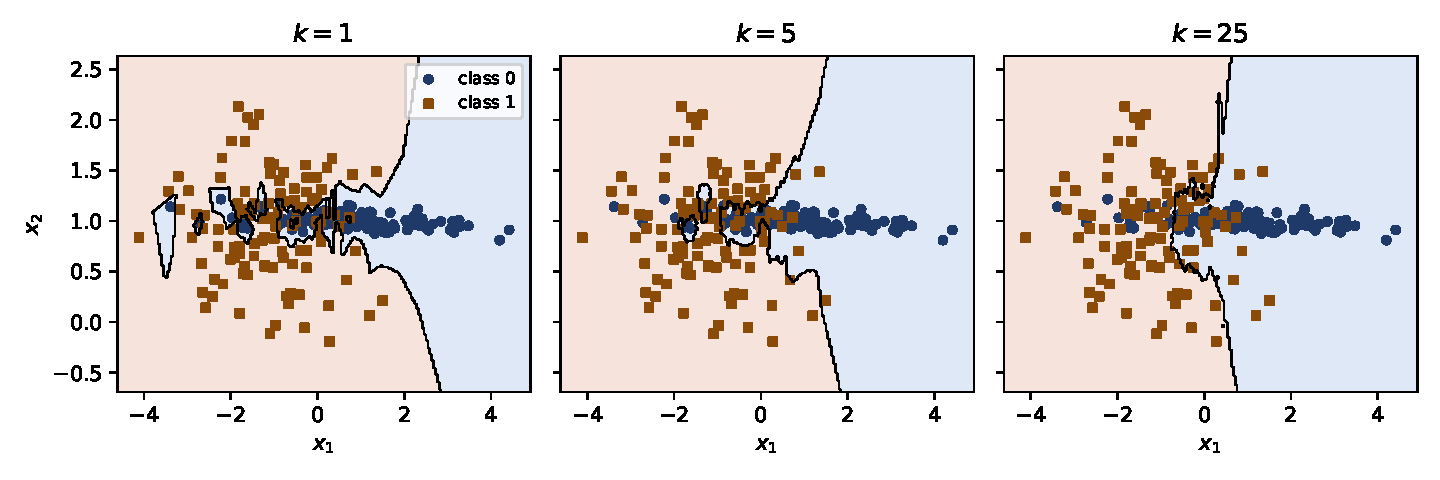
\includegraphics[width=\linewidth]{figures/ch03/knn_boundaries.pdf}
\caption{Decision boundaries at $k{=}1,5,25$ on two-feature synthetic data
(\texttt{figures/fig\_ch03\_knn\_boundaries.py}). $k{=}1$ traces every bump;
$k{=}25$ draws a nearly straight frontier; $k{=}5$ is the compromise that
usually wins.}\label{fig:knnbound}
\end{figure}

\section{Na\"ive Bayes: multiply small probabilities}\label{sec:nb}

Bayes' rule gives the probability of class $c$ given features $\mathbf{x}$:
$P(c \mid \mathbf{x}) \propto P(c)\,P(\mathbf{x} \mid c)$. Na\"ive Bayes
assumes conditional independence ---
$P(\mathbf{x}\mid c) \approx \prod_j P(x_j \mid c)$ --- turning a $d$-way
joint density into $d$ independent one-way densities you can estimate from
counts or Gaussians. The assumption is wrong almost always and useful
surprisingly often\index{conditional independence}.

Two engineering details matter. Likelihoods multiply to astronomically small
numbers, so work in \emph{log-space}: multiply becomes add, underflow becomes
harmless. And Gaussian likelihoods need a variance floor ($+\varepsilon$) or
a constant column produces a division by zero.

\lstinputlisting[language=Python,caption={\texttt{code/ch03/nb\_scratch.py}: Gaussian + categorical na\"ive Bayes in log-space on \texttt{titanic} ($700$ train / $191$ test).},label={lst:nb}]{code/ch03/nb_scratch.py}

\lstinputlisting[numbers=none]{code/ch03/nb_scratch.out.txt}

\begin{example}[WE 3.2 --- The confusion matrix by hand]\label{ex:nb}
Strategy: accuracy is one cell of a $2{\times}2$ story; read all four.\par
\begin{solution}
Listing~\ref{lst:nb} outputs $tp{=}48$, $fp{=}22$, $fn{=}24$, $tn{=}97$.
Accuracy $(48{+}97)/191 = 0.759$. Precision $48/(48{+}22) = 0.686$: of
everyone NB flags as a survivor, two-thirds really survived. Recall
$48/(48{+}24) = 0.667$: it misses one-third of actual survivors. Same
model, three different reputations --- which one is ``good'' depends on
whether you are allocating lifeboats or writing a newspaper.
\end{solution}
\end{example}

\section{The split, and why it is touched once}\label{sec:split}

The default protocol: \emph{stratified} 80/20 split --- train on $80\%$,
holding the class ratio fixed in both halves, then score on $20\%$.
Stratification is not cosmetic: on a $99{:}1$ problem an unlucky random
split can put almost all positives in one half, and you learn a lie about a
model that never had a chance. Listing~\ref{lst:eval} is the book's
canonical harness; every later chapter calls something shaped exactly like
it.

\lstinputlisting[language=Python,caption={\texttt{code/ch03/eval\_protocol.py}: stratified split, logistic fit, confusion-based metrics on \texttt{breast\_cancer}.},label={lst:eval}]{code/ch03/eval_protocol.py}

\lstinputlisting[numbers=none]{code/ch03/eval_protocol.out.txt}

\section{Cross-validation}\label{sec:cv}

One split is one draw from a lottery --- run it again with a different seed
and the score moves by a point or two for free. $k$-fold
cross-validation\index{cross-validation} prices the model properly:
partition $\mathcal D$ into $k$ folds, take turns training on $k{-}1$ and
scoring on the held-out one, then report mean $\pm$ sd across the $k$
scores. The $5$-fold or $10$-fold mean is a better estimate of generalisation
than any single split; the sd tells you how much the estimate would wobble
under re-sampling.

Three variants earn their keep:

\begin{itemize}
\item \emph{Stratified}: preserve the class ratio per fold --- always on
  imbalanced data.
\item \emph{Grouped} (\texttt{GroupKFold}): keep all rows from one
  group --- patient, hospital, user --- in one fold. Without it, near-duplicate
  rows of the same entity straddle the boundary and the score leaks.
\item \emph{Time-aware}: score each fold on data \emph{later} than its
  training window --- the only honest choice when the row order is a
  timestamp; random folds let the future train the past.
\end{itemize}

CV costs $k$ refits and still spends its test meaning a little every time
you tune on it: once you have chosen hyperparameters by CV, the honest
protocol is a \emph{final} untouched test set.

\section{Metrics for regression}\label{sec:regmetrics}

For regression, four error names recur; know what each pays attention to.

\begin{itemize}
\item $\mathrm{MAE} = \frac{1}{n}\sum |y_i - \hat y_i|$ --- the mean
  miss; robust, interpretable, in the units of $y$.
\item $\mathrm{MSE} = \frac{1}{n}\sum (y_i - \hat y_i)^2$ --- penalises
  big misses quadratically; smooth for optimisation.
\item $\mathrm{RMSE} = \sqrt{\mathrm{MSE}}$ --- back in $y$'s units while
  keeping the quadratic taste.
\item $R^2 = 1 - \frac{\sum(y_i-\hat y_i)^2}{\sum(y_i-\bar y)^2}$ --- the
  fraction of variance explained; $1$ perfect, $0$ means you tied the
  constant-mean model, negative means you did \emph{worse} than predicting
  the average.
\end{itemize}

\begin{checkpoint}[A number that needs a baseline]
$R^2$'s definition reveals a habit worth keeping: \emph{every metric needs
a stated baseline}. $0.90$ is brilliant against the mean and embarrassing
against last year's model. Quote the baseline alongside the score or the
score is marketing.
\end{checkpoint}

\section{Metrics for classification}\label{sec:clsmetrics}

\begin{figure}[ht]\centering
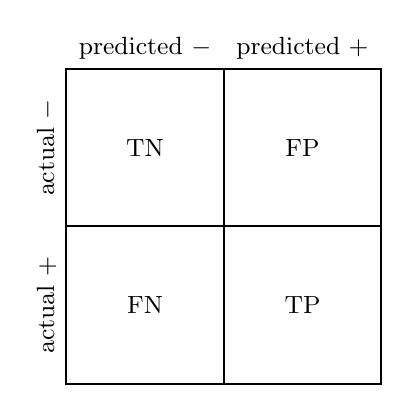
\begin{tikzpicture}[font=\small]
  \draw[thick] (0,0) rectangle (4,4);
  \draw[thick] (2,0) -- (2,4); \draw[thick] (0,2) -- (4,2);
  \node at (1,3) {TN};
  \node at (3,3) {FP};
  \node at (1,1) {FN};
  \node at (3,1) {TP};
  \node[above] at (1,4) {predicted $-$};
  \node[above] at (3,4) {predicted $+$};
  \node[left, rotate=90, anchor=south] at (0,3) {actual $-$};
  \node[left, rotate=90, anchor=south] at (0,1) {actual $+$};
\end{tikzpicture}
\caption{The confusion matrix\index{confusion matrix}: the four numbers
every classification metric is made of. Rows are truth, columns are
predictions.}\label{fig:confmat}
\end{figure}

Everything in the section is algebra on the four cells of
Figure~\ref{fig:confmat}:
\begin{align*}
\text{accuracy}  &= \frac{tp+tn}{tp+fp+fn+tn} &
\text{precision} &= \frac{tp}{tp+fp} &
\text{recall}    &= \frac{tp}{tp+fn} \\[2pt]
\text{FPR}       &= \frac{fp}{fp+tn} &
\text{TPR}       &= \text{recall} &
F_1              &= \frac{2\,P\,R}{P+R}
\end{align*}

Precision\index{precision} and recall\index{recall} trade off through the
decision threshold: raise it and precision climbs while recall falls. ROC
curves\index{ROC} trace all thresholds at once --- TPR vs FPR --- and AUC
summarises the whole trade-off as one number ($0.5$ is chance, $1.0$ is
perfect, $0.995$ on our \texttt{breast\_cancer} split). When classes are
imbalanced, accuracy becomes a con: predicting everyone benign on a
$62.6\%$-benign set already scores $0.632$. The chapter's rule of thumb:
on imbalanced problems lead with $F_1$, precision, and recall --- and
always name the lazy baseline.

\begin{figure}[ht]\centering
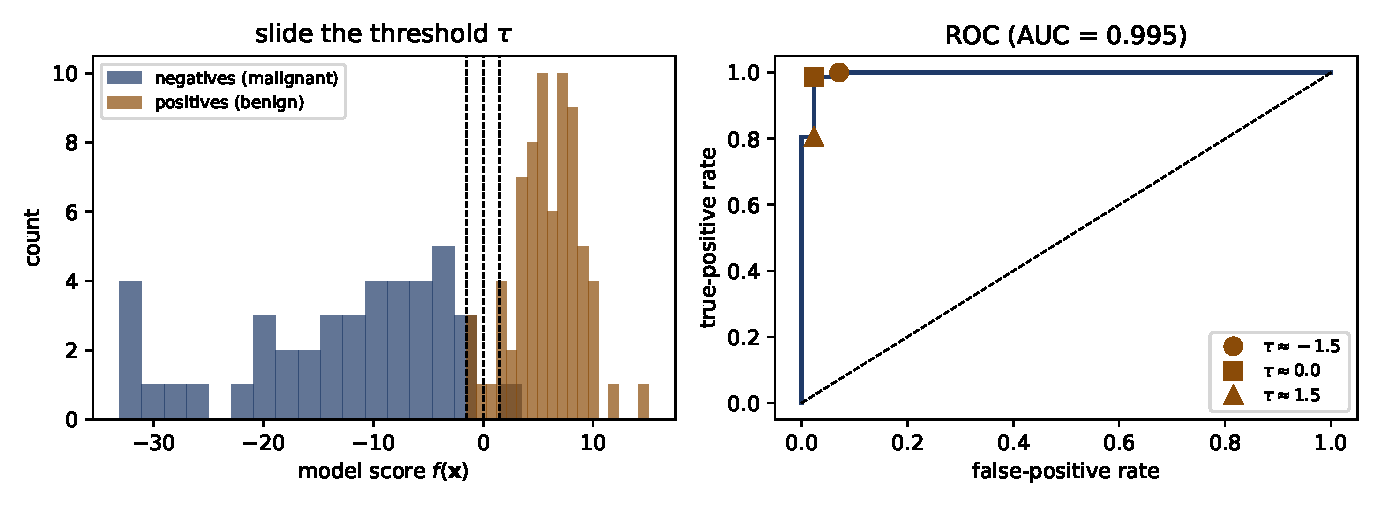
\includegraphics[width=\linewidth]{figures/ch03/roc_steps.pdf}
\caption{ROC construction (\texttt{figures/fig\_ch03\_roc\_steps.py}): a
threshold sweeps the score distribution (left); each threshold produces one
(FPR, TPR) point (right). AUC $=0.995$ measured on
\texttt{breast\_cancer}.}\label{fig:roc}
\end{figure}

\section{Bias, variance, and the learning curve}\label{sec:biasvar}

\begin{definition}[Bias and variance]\index{bias}\index{variance}
\emph{Bias} is systematic error --- the model is too simple to express the
pattern (underfit). \emph{Variance} is instability --- the model is so
flexible it reshapes itself to noise (overfit). Diagnose the pair from the
train--test gap: big gap, variance; both bad, bias.
\end{definition}

\begin{figure}[ht]\centering
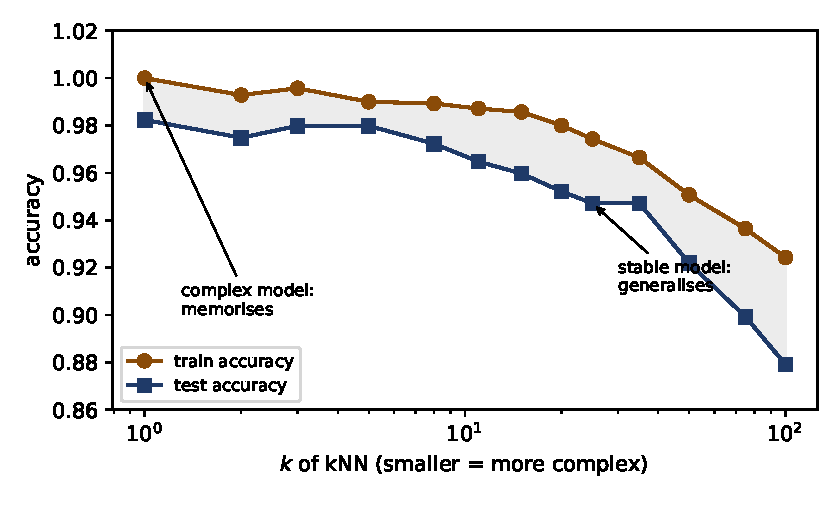
\includegraphics[width=0.72\linewidth]{figures/ch03/biasvariance.pdf}
\caption{Train vs test accuracy as $k$ of kNN varies
(\texttt{figures/fig\_ch03\_biasvariance.py}): the grey wedge is the
generalisation gap. Complexity lives at the left --- $k{=}1$ memorises
perfectly and generalises worst.}\label{fig:biasvar}
\end{figure}

The learning curve\index{learning curve} --- accuracy against training-set
size --- tells you which medicine to take. If the two curves still converge
as data grows, more data helps (variance-limited); if they have both
plateaued at a mediocre level, more data is wasted effort (bias-limited ---
get features or a better model family, not more rows).

\begin{figure}[ht]\centering
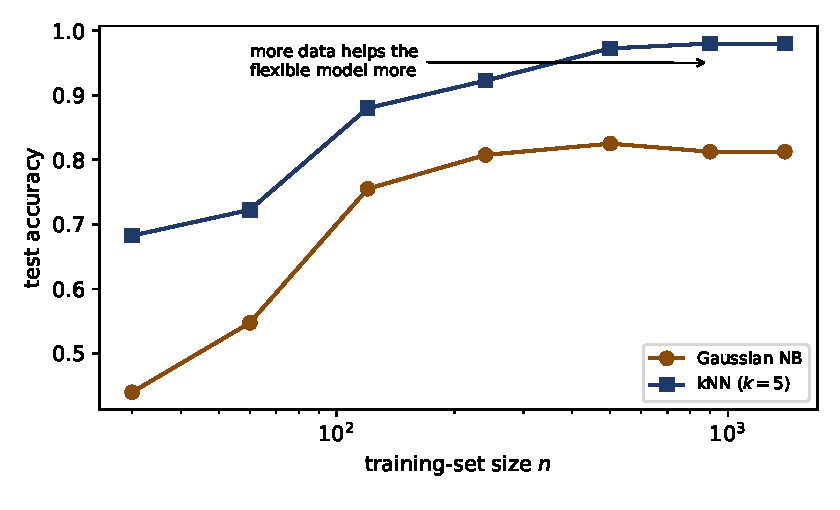
\includegraphics[width=0.72\linewidth]{figures/ch03/learning_curve.pdf}
\caption{Learning curves on \texttt{digits}
(\texttt{figures/fig\_ch03\_learning\_curve.py}). Gaussian NB plateaus near
$0.81$--$0.83$ --- its independence assumption is a bias ceiling more data
cannot break. 5-NN keeps climbing: $0.68 \to 0.88 \to 0.97 \to 0.98$ at
$n=30,120,500,1397$.}\label{fig:learncurve}
\end{figure}

\begin{example}[WE 3.3 --- Which medicine?]\label{ex:whichmedicine}
Strategy: the shape of the learning curve picks the remedy.\par
\begin{solution}
Figure~\ref{fig:learncurve} shows NB flattening by $n{\approx}500$: its
plateau is bias, so add a model family (trees, linear models), not rows.
5-NN at $n{=}1397$ still has a rising slope --- spend effort collecting
more data or running CV to pick $k$, and the score should keep improving.
Diagnose the plateau \emph{before} you collect --- collecting is the most
expensive fix.
\end{solution}
\end{example}

\section{Leakage: the five ways it sneaks in}\label{sec:leakage}

\index{leakage}Leakage is test information --- or future information, or
the label itself --- reaching the model at training time. It does not
announce itself; it looks like a great score. Five recurring routes:

\begin{enumerate}
\item \emph{Duplicate or near-duplicate rows} across the boundary
  (Chapter 1's fake win).
\item \emph{Preprocessing before the split} --- a scaler, imputer, or
  feature-selector that read the test rows.
\item \emph{Group bleed} --- siblings of the same patient/user/day on both
  sides; solved by grouped splits.
\item \emph{Target-encoded features} computed on the full data --- the
  encoding literally contains the test labels.
\item \emph{Time leakage} --- features computed with a window reaching
  past the prediction timestamp.
\end{enumerate}

\lstinputlisting[language=Python,caption={\texttt{code/ch03/leak\_demo.py}: two leaks, two sizes --- and the honest measurement that leak size \emph{depends on how much test information the step consumed}.},label={lst:leakdemo}]{code/ch03/leak_demo.py}

\lstinputlisting[numbers=none]{code/ch03/leak_demo.out.txt}

\begin{example}[WE 3.4 --- Leak autopsy]\label{ex:leakdemo}
Strategy: run the leak and the honest protocol side by side; measure the
phantom instead of assuming it.\par
\begin{solution}
Protocol (a) is the textbook ``scale on everything first'' leak --- and on
this clean iid data it \emph{loses} $0.9$\,pp rather than gaining. The
lesson is the finer one: a mild leak's size is proportional to how much
test information the leaked statistic absorbed, and on iid splits that is
nearly nothing --- which is exactly why mild leaks are dangerous, they
hide. Protocol (b) shows the leak at full strength: copying half the test
set into training buys 1-NN a free $+4.4$\,pp ($0.921 \to 0.965$). Same
mechanism, different doses --- every leak is the model peeking at an
answer key, and the score stops meaning what it says.
\end{solution}
\end{example}

\begin{example}[WE 3.5 --- The imbalance rerun]\label{ex:imbalance}
Strategy: ask ``good compared to what?'' and build the lazy classifier the
score must beat.\par
\begin{solution}
On \texttt{breast\_cancer} a logistic regression scores $0.956$ accuracy ---
sounding great until the lazy ``everyone benign'' model scores $0.632$
without touching a feature. The model's real margin is the gap, and the
honest metrics are precision $0.986$, recall $0.944$, $F_1=0.965$: of
$72$ true positives it caught $68$ --- the $4$ misses are the $4$ diagnoses
the metric was invented to count. On a $99{:}1$ problem the lazy baseline
scores $0.990$ and accuracy alone tells you nothing at all.
\end{solution}
\end{example}

\begin{wins}
What you can now do: state the supervised frame ($\mathcal D$, $f_\theta$,
loss, split, metric) and recite why the test set is sealed; implement kNN
and na\"ive Bayes from scratch and read a $k$-sweep for bias/variance;
build stratified, grouped, and time-aware CV; compute the confusion quartet
and choose the right metric under imbalance; diagnose plateau shape on a
learning curve; autopsy a leak by measuring the phantom.
\end{wins}

\section{Common mistakes}

\begin{description}
\item[Tuning on the test set] Every peek spends meaning. Tune on
  train+CV; the test set hears about your choices only after they are
  frozen.
\item[Preprocessing before the split] Fit scalers, imputers, and
  encoders on train only; inside CV, refit them inside each fold --- a
  pipeline object exists precisely so you cannot forget.
\item[Trusting accuracy on imbalance] A $0.99$ score on a $99{:}1$
  problem is the lazy classifier wearing a costume. Report precision,
  recall, $F_1$ --- and always the lazy baseline.
\item[Random folds on grouped or timed data] Siblings of the same entity
  straddle the boundary, or the future trains the past. Use
  \texttt{GroupKFold} or a time-ordered split.
\item[Reading one split as the truth] A single 80/20 score is one lottery
  draw. CV mean $\pm$ sd is the honest number.
\item[Micro-averaging away the small class] Overall accuracy or
  micro-$F_1$ can rise while the minority class is missed entirely ---
  report per-class recall too.
\item[Skipping the baseline] Every score needs a named baseline next to
  it --- mean predictor, majority class, last year's model. Without one
  the score is a number without a denominator.
\item[$k$ too small] $k{=}1$ wins every training argument and loses the
  deployment. Read the sweep, not just the peak.
\item[Probability out of thin air] Na\"ive Bayes without the log-space
  fix underflows to zero and returns the wrong argmax --- multiply
  probabilities only inside \texttt{log}.
\end{description}

\section{Summary table}

\begin{tabularx}{\linewidth}{@{}l l X@{}}
\toprule
\textbf{Idea} & \textbf{Tool} & \textbf{When to reach for it}\\
\midrule
Supervised frame & $\mathcal D, f_\theta$, loss, split & every problem --- state it first\\
kNN & \texttt{KNeighborsClassifier} & small-$n$ baseline; distances meaningful\\
Na\"ive Bayes & log-space likelihoods & fast baseline; sparse/high-$d$ text\\
Split & stratified 80/20 & the default single evaluation\\
CV & $k$-fold, stratified/grouped/time & the honest score for tuning\\
Regression metrics & MAE, RMSE, $R^2$ & error size vs variance explained\\
Classification metrics & P/R/$F_1$, ROC-AUC & imbalance; threshold trade-offs\\
Bias--variance & train--test gap, learning curve & pick medicine: data vs features\\
Leakage & five routes checklist & every pipeline, before quoting a score\\
\bottomrule
\end{tabularx}

\section{Drill --- five concept questions}

\begin{enumerate}
\item $k{=}1$ gives perfect train accuracy. Which of bias or variance is
  at work, and what does the train--test gap measure?
\item Name two splits that beat a random 80/20 when rows come from
  patients or timestamps.
\item On $99{:}1$ imbalance, accuracy reads $0.991$ and $F_1$ reads
  $0.45$. Which model is better than chance?
\item A scaler fitted on all rows inflates accuracy by $0.4$\,pp on one
  dataset and $40$\,pp on another. What differs?
\item NB plateaus on the learning curve. Data, features, or $k$ --- which
  knob do you turn?
\end{enumerate}

\section*{Further reading}
\begin{itemize}
\item Hastie, Tibshirani \& Friedman --- \emph{The Elements of Statistical
  Learning} (book site; free PDF under ``Download the book PDF'').
  \url{https://hastie.su.domains/ElemStatLearn/} --- ch.~2 (bias--variance)
  and ch.~7 (model assessment) are this chapter's graduate ancestor.
  \index{ESL}
\item scikit-learn --- \emph{Model evaluation}.
  \url{https://scikit-learn.org/stable/modules/model_evaluation.html} ---
  the reference for every metric used here, with the same naming.
\item scikit-learn --- \emph{Cross-validation}.
  \url{https://scikit-learn.org/stable/modules/cross_validation.html} ---
  fold splitters incl.\ \texttt{StratifiedKFold}, \texttt{GroupKFold},
  \texttt{TimeSeriesSplit}.
\item scikit-learn --- \emph{Common pitfalls}.
  \url{https://scikit-learn.org/stable/common_pitfalls.html} --- the
  library's own leakage catalogue; our five routes are its headliners.
\item Cawley \& Talbot, ``On Over-fitting in Model Selection and Subsequent
  Selection Bias in Performance Evaluation,'' \emph{JMLR} 11 (2010).
  \url{https://www.jmlr.org/papers/v11/cawley10a.html} --- what tuning on
  the test score costs, measured.
\item Domingos, ``A Few Useful Things to Know about Machine Learning,''
  \emph{CACM} 55(10), 2012.
  \url{https://homes.cs.washington.edu/~pedrod/papers/cacm12.pdf} ---
  the classic aphorisms; ``generalisation'' is item one.
\item Fawcett, ``An introduction to ROC analysis,'' \emph{Pattern
  Recognition Letters} 27 (2006).
  \url{https://people.inf.elte.hu/kiss/11dwhdm/roc.pdf} --- the canonical
  ROC tutorial behind Figure~\ref{fig:roc}.
\item scikit-learn --- \texttt{confusion\_matrix} API.
  \url{https://scikit-learn.org/stable/modules/generated/sklearn.metrics.confusion_matrix.html}
  --- row/column convention used throughout the book.
\end{itemize}

\begin{rulebox}{Watch instead (if you'd rather see it)}
\begin{itemize}
\item \textbf{StatQuest: Machine Learning Fundamentals --- The Confusion
  Matrix} (7:12). StatQuest with Josh Starmer.
  \url{https://www.youtube.com/watch?v=Kdsp6soqA7o} --- the four cells
  animated with the same row/column convention as
  Figure~\ref{fig:confmat}; matches \S\ref{sec:clsmetrics}. Accessed
  2026-10-11.
\item \textbf{StatQuest: Machine Learning Fundamentals --- Cross
  Validation} (6:04). StatQuest with Josh Starmer.
  \url{https://www.youtube.com/watch?v=fSytzGwwBVw} --- fold diagrams and
  the why; matches \S\ref{sec:cv}. Accessed 2026-10-11.
\item \textbf{StatQuest: ROC and AUC, Clearly Explained!} (16:17).
  StatQuest with Josh Starmer.
  \url{https://www.youtube.com/watch?v=4jRBRDbJemM} --- threshold-sweep
  construction matching Figure~\ref{fig:roc}; matches
  \S\ref{sec:clsmetrics}. Accessed 2026-10-11.
\end{itemize}
\end{rulebox}

\chapternotes
\begin{enumerate}
\item The $k$-NN expansion $\|\mathbf{a}-\mathbf{b}\|^2 =
  \|\mathbf{a}\|^2 - 2\mathbf{a}^T\mathbf{b} + \|\mathbf{b}\|^2$ is the
  standard trick; in higher dimensions an index (KD-tree, ball tree, or
  an approximate index like HNSW) replaces the brute-force product.
\item Na\"ive Bayes's independence assumption is violated constantly and
  still ranks among the best first baselines on sparse text --- see
  Domingos \& Pazzani (1997) for why the ranking survives even when the
  probabilities do not~\cite{domingos1997}.
\item ``The test set is touched once'' is the ideal; in practice the
  budget is a small integer. See Cawley \& Talbot (2010) in Further
  reading for the measured cost of each extra peek.
\item \texttt{GroupKFold} and \texttt{TimeSeriesSplit} documentation and
  examples are under the sklearn cross-validation page cited in Further
  reading.
\item The phantom-leak magnitudes here were measured on
  \texttt{breast\_cancer} (random state 7); the direction is the lesson,
  not the digits --- rerun \texttt{leak\_demo.py} with other seeds and
  the qualitative pattern holds.
\end{enumerate}

\section*{Exercises}

\emph{[easy]}
\begin{exercise}
Compute precision, recall, and $F_1$ by hand for
$tp{=}30$, $fp{=}10$, $fn{=}20$, $tn{=}140$.
\end{exercise}
\begin{exercise}
A classifier scores $0.97$ accuracy on a $30{:}1$ imbalanced set where
the majority class is $96.8\%$ of rows. Is it better than the lazy
classifier? What would $F_1$ of the lazy classifier be?
\end{exercise}
\begin{exercise}
In $5$-fold CV on $n{=}800$, how many rows does each fold's test split
hold, and how many total refits happen?
\end{exercise}
\begin{exercise}
Why does $R^2{=}0$ not mean ``the model predicts zero''? What does it
predict instead?
\end{exercise}
\begin{exercise}
Which is bigger at $k{=}1$: train accuracy or test accuracy? What
closes the gap as $k$ grows?
\end{exercise}

\emph{[medium]}
\begin{exercise}
Implement \texttt{stratified\_split} \texttt{(y, test\_frac, seed)} from
scratch: group indices by class, shuffle each group, carve each at the
same fraction. Verify class ratios match on \texttt{titanic.survived}.
\end{exercise}
\begin{exercise}
Extend Listing~\ref{lst:eval} to print micro-\emph{and} macro-$F_1$ on
\texttt{digits}. Which classes lose the most under macro averaging?
\end{exercise}
\begin{exercise}
Make the grouped-split argument concrete: split \texttt{titanic} by
\texttt{ticket} number as the group key (\texttt{GroupKFold} with
\texttt{groups=df.ticket}) and compare kNN test accuracy vs a plain
random split. Which is higher, and why does that hurt?
\end{exercise}
\begin{exercise}
Sweep the classification threshold of a logistic model on
\texttt{breast\_cancer} from $0.1$ to $0.9$; plot precision and recall
against it and mark the $F_1$-maximising threshold.
\end{exercise}
\begin{exercise}
Re-run Listing~\ref{lst:leakdemo} on \texttt{digits} instead of
\texttt{breast\_cancer}. Does the scale-then-split phantom grow, shrink,
or flip sign? Explain with the ``how much test information'' rule.
\end{exercise}
\begin{exercise}
Write \texttt{sliding\_window\_cv(X, y, k)} that yields (train, test)
index pairs where each test fold is strictly later than its train fold.
\end{exercise}

\emph{[hard]}
\begin{exercise}
Prove that the NB decision boundary between two classes is linear when
both class-conditionals are Gaussian with \emph{equal} variances, and
quadratic when they differ. (Hint: set the two log-posteriors equal and
collect terms.)
\end{exercise}
\begin{exercise}
Derive why accuracy fails at $99{:}1$ imbalance: give the largest
accuracy achievable by a classifier whose recall on the minority class
is $r$, and show it is maximised at $r{=}0$.
\end{exercise}
\begin{exercise}
Design a leak-free grouped split for a dataset with two grouping keys
(family \emph{and} cabin) --- prove no group straddles the boundary in
either key, or explain why you cannot satisfy both and must pick one.
\end{exercise}
\begin{exercise}
Show that under squared loss, the best constant predictor of $y$ is
$\bar y$ --- and that this is exactly what $R^2{=}0$ measures.
\end{exercise}
\begin{exercise}
A friend reports ``$0.99$ ROC-AUC'' on a dataset that contains the same
patient's two scans split across train/test. Reproduce a version of the
bug on \texttt{titanic} using \texttt{ticket} as the group, and quantify
the inflation.
\end{exercise}

\section*{Hints and answers}
\begin{description}
\item[3.1] $P{=}0.75$, $R{=}0.60$, $F_1{=}0.667$.
\item[3.2] No --- lazy accuracy is $0.968$; lazy $F_1{=}0$ (no positive
  predictions). Report recall.
\item[3.3] $160$ rows per test fold; $5$ refits.
\item[3.4] It predicts $\bar y$ --- the constant-mean model is the $R^2{=}0$
  baseline.
\item[3.5] Train. Variance shrinks as neighbours vote; the gap closes.
\item[3.6] \texttt{np.argsort} inside a per-class loop; assert
  \texttt{np.isclose} on the two ratios.
\item[3.7] Macro-$F_1$ weights each class equally; rare digits show the
  bigger drop.
\item[3.8] Random split is usually higher --- sibling passengers share
  tickets; the model memorised family outcomes.
\item[3.9] Threshold $\uparrow$ $\Rightarrow$ precision $\uparrow$, recall
  $\downarrow$; the $F_1$ peak is typically around $0.4$--$0.6$ here.
\item[3.10] Tiny either way --- iid rows share statistics.
\item[3.11] Sort by time; fold $i$ tests on block $i{+}1$, trains on
  blocks $1..i$.
\item[3.12] Equal $\sigma^2$ $\Rightarrow$ the $x^2$ terms cancel in the
  difference of log-posteriors, leaving a linear form $w^Tx + b$.
\item[3.13] Accuracy $= 0.99 + 0.01\cdot(r - \text{FPR})$-ish; derive
  exactly and show the maximum over $r$ is at the corner.
\item[3.14] If any family spans cabins, one key must win --- pick the key
  with the stronger causal claim to leakage.
\item[3.15] Expand $\sum(y_i - c)^2$ and set the derivative in $c$ to
  zero.
\item[3.16] Grouped fold drops the apparent AUC to the honest level ---
  the inflation is the gap between the two protocols.
\end{description}
